\section{Drug delivery: challenges and solutions}

\subsection{Environmental challenges of drug delivery}
The problem of drug delivery is an excellent example of the hurdles existing between a theoretical model and nature: a new drug is usually designed to affect a specific target. Even if in silico experiment can prove the efficacy, its usefulness is bound to the ability to cross the barriers dividing the inoculation site from the specific target inside the human body.
%
To reach the aimed organ, drug molecules must be compatible with the different cellular environments they cross, but be preferentially retained from, and act only on, the ones they are designed for. This implies a subtle balance between a disruptive activity on one side, and harmlessness on the other, least the compound is recognised as dangerous and disposed of by the efficient immune and reticuloendothelial systems of the body, which aim at neutralise exogenous substances.

As en example, the trip of an orally  administered small molecule ``free" drug, i.e.\ an active molecule without any aiding delivery agent, passes through the digestive system, with its challenging acidic environment and limited permeation across the intestinal epithelium, and from there to the blood stream \cite{Masaoka2006, Mitragotri2014}. The drug then diffuses in the tissues flanking the blood vessels naturally depleting its concentration downstream \cite{Krol2012}, so that regions further away in the line have less chances of getting a sizeable dose. This implies that high drug concentrations might be needed at the starting point to efficiently target every organ.

However, this naive picture of drug diffusion is complicated by the impermeability of specific tissues: the brain for example, one of the most delicate organs in the body, is well protected from the attack of external agents by the blood brain barrier (BBB), which allows the passage of small molecules only ($<$ 400-500 Da, while standard ``small molecule drugs" weigh up to 900 Da), and only if they have high lipid solubility \cite{Pattni2015, Krol2012}. Other tissues, like tumoral ones, are instead poorly vasculated, reducing the chances of delivery at their interior \cite{Pattni2015}.

Moreover, as already hinted, during its journey to reach the receptor, enzyme or organelle it is meant for, a drug must not be sequestered by the immune systems. Many inorganic small molecules are not mimetic by themselves, i.e.\ often they do not resemble the ones naturally present in the body, and this brings uncertainty on how they would interact with the, for example, the components of the blood stream. Generally, as soon as they reach it, small molecules are coated by a protein corona based on their shape and charge \cite{Krol2012}. Such modifications are difficult to predict and can disrupt or decrease significantly the efficacy of a compound as they modify the way drugs are recognised and absorbed by the target. 

For all the above reasons, research has focussed on developing systems to assist the delivery of drugs \cite{Jain2016, Pattni2015, Mitragotri2014}. A mimetic carrier can not only improve delivery, but also be designed to selectively bind to particular tissues or to trigger a delayed drug release time or upon changes in environmental variables (for example pH) to reduce drug concentration in non targeted regions. A stand alone field of research has then focussed on the development of delivery vehicles irrespective from the quest for new drugs. The optimised products of the two separate efforts can then be paired according to the condition to address, to give a successful therapy.

At present, many molecules have been successfully employed to build drug vehicles: inorganic metals, polymers, lipids and proteins are all suitable for the aim and offer a range of different physico-chemical characteristics useful to target different cells \cite{Hughes2005} (Figure \ref{fig:vehicles}). A brief (and non exhaustive) overview of some of them is meaningful to point out the broad variety and exoticity of structures which are useful, sometimes unexpectedly, to the medical world.


\subsection{Inorganic materials for small drugs delivery}

\paragraph{Metal nanoparticles} In the range of inorganic compounds, golden nanoparticles demonstrated to be remarkably useful for tumour treatment: their structure can be customised in shape and size (down to a 10 nm radius), made less visible to the immune system by coating with biologically active moieties or conjugation to a poly-ethyleneglycol (PEG) polymer layer \cite{Singh2018}. From their metallic nature, golden nanoparticles inherit optical properties that allow to track them inside the body and to thermally stimulate them to trigger drug release, favouring the penetration through cell membrane or disrupting the nearby cells \cite{Boisselier2009}. This is important for tumour treatment because of the difficulty with which tumoural cells are reached by drugs and the selectivity required when delivering a highly damaging chemotherapeutic.

At present, there are mixed evidence about their toxicity \cite{Boisselier2009} and doubts have been raised on the long term effects of metallic fragments in the body. For that reason, only a few golden nanoparticle based compounds have made to the clinical stage so far \cite{Singh2018} but, given their high and still unexplored potential, they continue to be a primary interest for the medical community and a very active research field.

\begin{figure}
\begin{center}
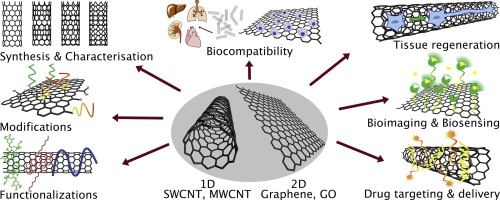
\includegraphics[width = 0.5\textwidth]{1introduction/pics/carbon_review.jpg}
\vspace{0.2cm}
\caption[Materials for drug delivery vehicles]{INCLUDE ONE EXAMPLE IMAGE (FROM PAPERS) FOR EACH MATERIAL (nanopartcles, carbon, polymers, lipids, DNA, proteins).} \label{fig:vehicles}
\end{center}
\end{figure}

\paragraph{Carbon nanotubes}
Similarly, carbon nanotubes have been used for biomedical applications as they have a high loading efficiency thanks to their high surface area and easy interaction with biomolecules through van der Waals interactions, $\pi$-$\pi$ stacking or hydrophobic effect \cite{Erol2017}. They are easy to functionalise through conjugation to extra organic groups to increase their biocompatibility and have potential for targeted drug release upon change in environmental pH \cite{Depan2011}.

Similarly to metallic nanoparticles, their applications are still at the experimental stage, with more verifications to be performed to give a viable product.


\paragraph{Polymers} Polymers are another large class of inorganic molecules functionalised for the benefit of medicine with several representatives already clinically approved as drug eccipients. For example, PEG, already mentioned as aid to make golden nanoparticles bio-compatible, it is widely used, thanks to its high hydrophilicity, to mimetise structures (e.g.\ inorganic nanoparticles, peptides) which in turn carry a drug \cite{Lammers2009}; or as a stand alone carrier system which has a high drug payload \cite{Liechty2010}. The great strength of polymers is their flexibility: as each of their constituent monomers can be either hydrophilic or hydrophobic, they can be engineered to assemble in many different structures \cite{Kawakatsu2004}. Moreover, they can trigger a sustained drug release by swelling slowly in water \cite{Nicolas2013}, or undergo sol-gel phase transition upon specific changes in the environment \cite{Liechty2010}. Finally, research has also focussed on improving their biodegradability \cite{Nair2007} and in making polymers a bioactive compound itself \cite{Rao2018}.


\subsection{Organic materials for small drugs delivery} \label{sec:organic}

A somehow opposite approach for designing drug vehicles consists in using molecules similar to the ones present in the body, in an effort to exploit already available biocompatible materials and reduce toxicity \cite{Yoo2011}. In this category fall lipids, DNA and peptides.

\paragraph{Lipids} Lipids are the main constituents of the cell membrane. They come with a great variety, broaden by the many species produced synthetically. The components selected for drug delivery are usually taken from the biological lipidome \cite{seeRebuttal}, but the composition of the final assembly differs from the one of cellular membranes, and possibly includes synthetic molecules, to tune the release properties and enable them to survive the delivery journey \cite{Yingchoncharoen2016}. For example, as mentioned for other materials, a change in pH can dissolve the lipid structure exposing its content.
%
Lipids can encapsulate efficiently both hydrophobic or hydrophilic drugs, arranging themselves respectively in micelles structures (monolayer spheres with the hydrophobic tails facing the interior) or in liposomes (bilayer spheres with a water filled core) \cite{Bunker2016}. By now, many of them overcame the clinical trials and are currently approved as delivery agents for cancer and infections drugs \cite{Pattni2015paper, Jain2017}.

\paragraph{DNA scaffolds} Similarly, many DNA scaffolds have been tested for smart delivery: DNA origami is nowadays an established technique to build three dimensional customised solids \cite{Linko2015}, and the nanometric knowledge about their constituents allows to fine tune them for a triggered release of the content \cite{Douglas2012}. First studies proved them successful in delivering anticancer agents \cite{Zhang2014, Jiang2012}, however they are very sensitive to different cellular environments which challenge their stability. This, united with high production costs and the relative young developments in their manipulation, prevented them to constitute a viable class of carriers so far, but at the same time holds promise for future improvements and applications.

\paragraph{Peptidic scaffolds} Another widely used and trustworthy mimetic vehicle comes, quite surprisingly, from the world of pathogens: viruses have co-evolved with humans, to be able to penetrate into cells where they complete their reproductive cycle \cite{Lobo2009}. Therefore their capsid, the peptidic shell encapsulating the genome, is highly suitable for cell penetration. The first application sought historically was to employ genome free viruses to stimulate and train the natural immune response against the respective genome-loaded ones, creating viral vaccines - in a concept similar to the inoculation of dead bacteria to counteract the infections caused from them \cite{Lauer2017}.
Later in the history, their potential as cargo carrier was pursued by first modifying the original genetic material to include sequences beneficial for the host cell, and inactivate the ones promoting the infectious duplication at the same time. In particular adeno-associated virus (AAV) has been widely studied \cite{Daya2008} as it triggers a low immune response \cite{Buning2015}, and the first AAV viral therapy has been approved a few years ago \cite{Smalley2017}.
%
To fully exploit the potential of a peptidic carrier many efforts have focussed on synthesising in vitro gene-free capsids, either as they appear in nature \cite{Wu2009} or designing artificial building blocks, which assemble in so called Virus-Like particles (VLPs). This helps overcoming the reaction stimulated by specific viral capsids to which the immune system is sensible to.
%
Similarly to other delivery vehicles, the surface of VLPs can be functionalised with additional molecules to improve the target selectivity and increase biocompatibility, while the capsid peptidic scaffold grants robustness to the structure. Therefore, VLPs loaded with drugs can be tuned for an efficient intra cellular release \cite{Ma2012}.

A step further in engineering peptidic structures is represented by the design of self-assembling functional structures from first principles, exploiting the physico-chemical characteristics of peptides, regardless their resemblance of viral capsids.
%
Indeed, self-assembling peptides can form nanostructures ranging from nanoparticles to nanotubes, nanofibers, nanorods and hydrogels \cite{Fan2017,Habibi2016}.
%
Among their advantages, peptides present biocompatibility, a low production cost and a tunable bioactivity thanks to their chemical diversity, which helps in tailor the assembly toward the target of interest \cite{Fan2017}. Moreover, the variety of amino acid available makes possible to load peptidic structures with both hydrophilic and hydrophobic drugs, according to their amino acid composition \cite{Habibi2016,Ma2012}.
%
The peptidic self-assembly is modulated by the peptide length and its hydrophobic or hydrophilic character, given by its amino acid composition: on one end of the length scale, phenylalanine dipeptides were designed with inspiration from a pathogenic pathway of molecular self-assembly \cite{Yan2010} and were shown to self-assemble in a multi-scale process producing nanotubes able to load drug molecules \cite{Silva2013}. The relatively small diphenylalanine building block is non the less complex as it bears two charged termini (as the process is observed at neutral pH), and two aromatic hydrophobic rings, so that the dipeptide is driven towards assembly by the hydrophobic forces acting on the phenylalanine side chains and the complementary charges of the termini.

In a different approach, longer sequences can be employed to guide the formation of the local structure, as they organise spatially in well studied motives (the secondary structure) with known interactions among themselves.
%
The two typical secondary structures, $\alpha$-helices and $\beta$-sheets, appear in sequences of about 20 or more amino acids length and both can be amphiphatic, thus promoting the assembly between the hydrophobic faces of different copies of the same structure. With the appearance of a secondary structure, more complex building blocks can be designed, to tune the shape into the ones needed for the supramolecular organisation of interest \cite{King2014}.
%
The easy manipulation of peptides is made possible because proteins are a fundamental,  well studied component of the human body: thus, the knowledge of many of their structures\cite{PDB} give an insight in how the small ones can hierarchically assemble into larger units.
%
Moreover, the vast literature on their interactions with membranes, cell receptors and in general biological components, can inspire the design of building blocks sensible to particular triggers within the body. From this background, the outlook of protein design often goes in the direction of surpassing natural limitations, synthesising exotic, non natural, geometries \cite{Yeates2019,Malay2019} for multifunctional materials.


\subsection{Mechanisms of antimicrobial resistance to small drugs} \label{sec:AMR_mechs}

Antimicrobial resistance can manifest through many different mechanisms, as highlighted in the example of the penicillin resistant bacteria.
%
In particular, resistance mechanisms fall into three main groups: a first group minimises intracellular concentration of the antibiotic preventing penetration or maximising efflux; a second one modifies the antibiotic target by genetic mutation or post-translational modification; finally a third group inactivates the antibiotic by hydrolysis or modification of the drug molecule (Figure \ref{fig:amr}) \cite{Blair2014}. We give here a brief review of them, to help understanding the pitfalls of existing drugs and the characteristics sought in the developments of new compounds.

\begin{figure}[h]
\begin{center}
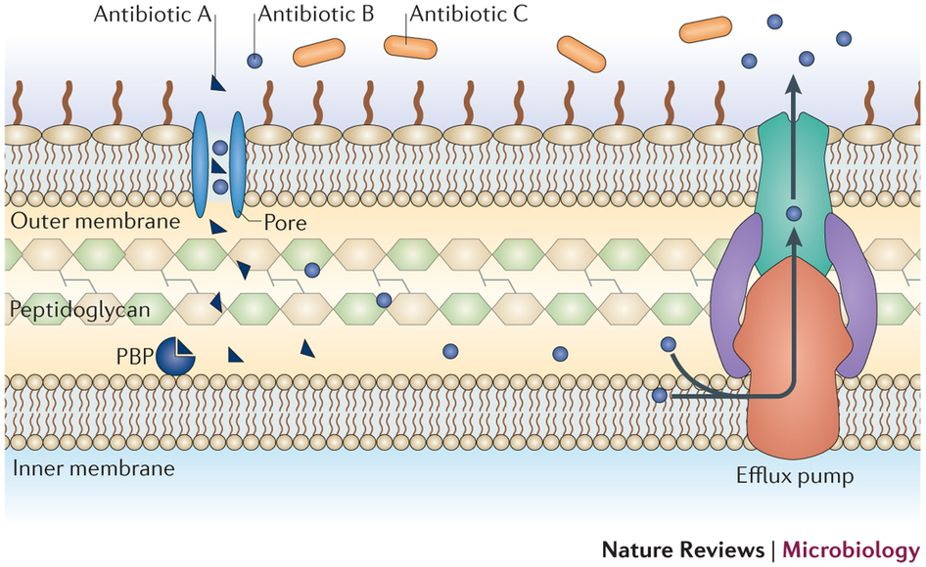
\includegraphics[width = 0.6\textwidth]{1introduction/pics/amr1}
\vspace{0.8cm}
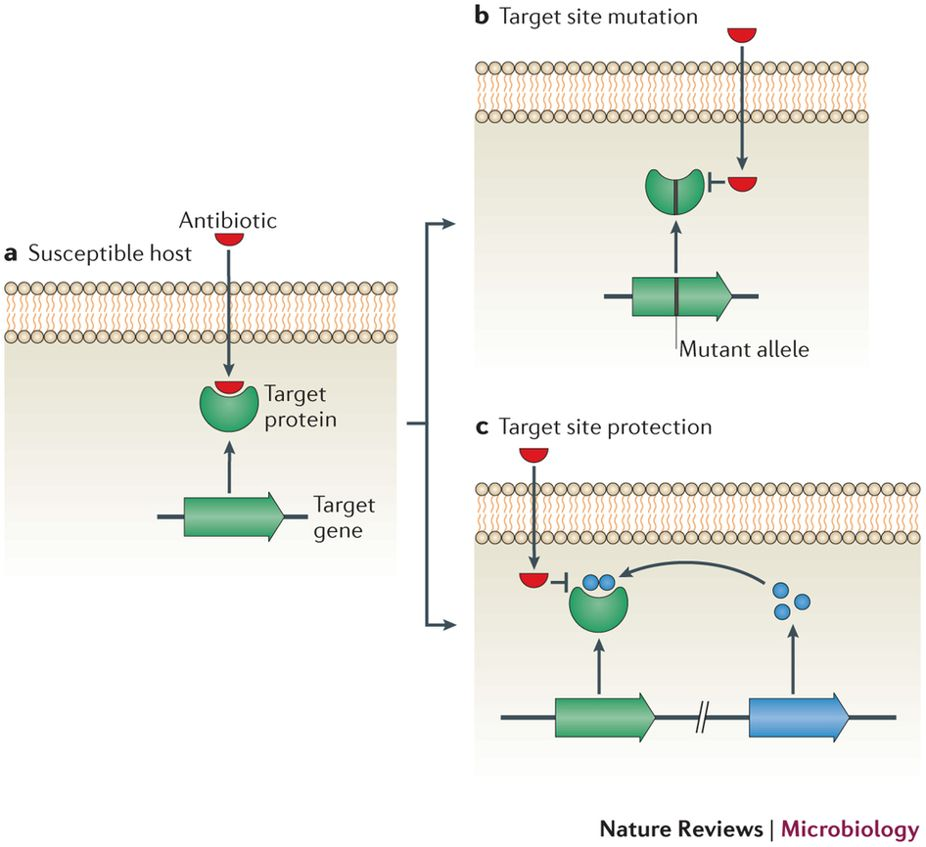
\includegraphics[height = 0.36\textheight]{1introduction/pics/amr3}
\hspace{0.5cm}
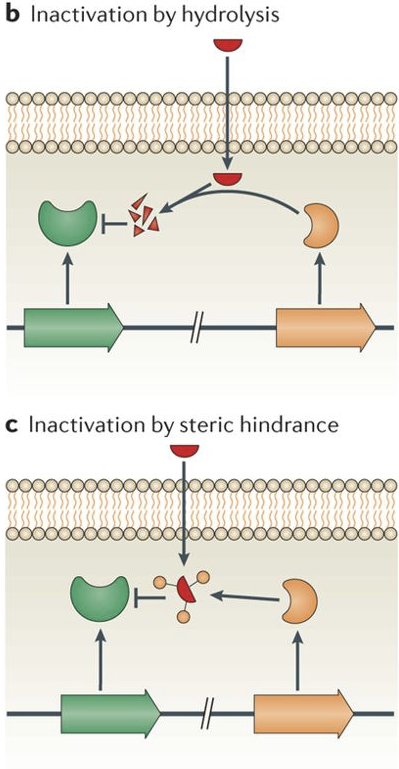
\includegraphics[height = 0.36\textheight]{1introduction/pics/amr4_half}
\caption[Mechanisms of antimicrobial resistance to small drugs]{Mechanisms of antimicrobial resistance to small drugs. a) Intrinsic mechanisms of resistance (removal of antibiotic B by efflux pump and inaccessibility of antibiotic C to the PBP target because of membrane impermeability). b) Target site change via mutation or protection. c) Direct interactions with antibiotics causing its disruption or structural modification. Reproduced from \cite{Blair2014}.} \label{fig:amr}
\end{center}
\end{figure}


\paragraph{Prevention of access to target}
One possible mechanism of defence bacteria employ against antibiotics is to prevent the access to the target. This is performed either blocking the drug influx or promoting its quick efflux in the eventuality it has entered the cell.

Regarding drug influx, not all the molecules can enter the cell permeating the membrane, and this holds particularly for hydrophilic antibiotics tackling Gram-negative bacteria: indeed, compared with Gram-positive ones, Gram-negative bacteria are intrinsically less permeable because of the structure of the additional outer membrane \cite{Delcour2009}, therefore hydrophilic molecules are imported into the cell through outer-membrane porin proteins \cite{Vargiu2012,Kojima2013} (for further details on the bacterial membrane structure, see Section \ref{sec:host-defense-peptides}).
%
The major porins of most Enterobacteriaceae are thought to be non-specific channels \cite{Tran2013}, therefore replacing porins with more selective channels or down regulating their expression would limit the intake of the drug. This last mechanism is well established and contribute to resistance to many different drugs in Gram-negative bacteria, including newer drugs such as carbapenems and cephalosporins, for which resistance is otherwise mediated by enzymatic degradation \cite{Tamber2003,Baroud2013,Lavigne2013,Poulou2013,Wozniak2012} (see the related paragraph below).
Alternatively, as happens in E. coli exposed to carbapenems, not only the porin expression is down-regulated, but also the genes coding for them are heavily mutated, suggesting that changes in the porin structure can enhance their selectivity and reduce the drug influx \cite{Lavigne2013,Novais2012,Tangden2013}.

A strategy complementary to prevent drug influx is to dispose the drug efficiently once it has invaded the cell. Bacterial efflux pumps transport many antibiotics out of the cell, and they constitute a major hurdle for the treatment of Gram-negative bacteria as opposed to Gram-positive ones. Indeed, many of the drugs effective on the latter are evacuated by the formers through efflux pumps; in particular, multidrug resistance (MDR) efflux pumps can transport a wide range of structurally dissimilar substrates.
%
All bacteria can produce their own MDR pumps \cite{Floyd2010,Hu2012,Kim2013,Ogawa2012}, but it has also been shown that some of the genes encoding for them have been transferred to plasmids and thus can be transferred to other bacterial species, disseminating resistance \cite{Dolejska2013}.

In general, the over-expression of efflux pump seen in multidrug-resistant bacteria is often due to mutation in the regulatory network controlling it, \cite{Abouzeed2008}, but it can also occur as a result of induction in response to environmental signals and in conditions in which their function is required \cite{Baucheron2014,Nikaido2011,Hirakawa2004}.


\paragraph{Change or modification of the antibiotic target}
Most antibiotics bind to the target with high affinity and therefore specificity. Small modifications of the target structure can disrupt an efficient binding of the antibiotic, still allowing the target to maintain its normal function. These modifications can be reached by either mutation or protection of the binding site.

In the first case, a casual mutation in  the genome would provide such minimal required change in the protein structure, and the resistant population would spread according to its improved fitness.
%
An example is the development of resistance to linezolid in S. pneumoniae and S. aureus: this drugs targets the 23S rRNA ribosomal subunit of Gram-positive bacteria which is encoded by multiple, identical copies of its gene. The use of linezolid has selected first a population with a mutation in one of the copies, which has afterwards passed to the other copies via recombination, generating a resistant population \cite{Billal2011,Gao2010}.
%
Other mutations occurred by transformation, i.e.\ uptake of DNA from the environment: in the case of penicillin resistant S. pneumoniae, a mutated penicillin-binding protein gene is included in the genome by recombination with DNA from the closely related species Streptococcus mitis. Similarly, the acquisition of a gene homologous resulted in a methicillin-resistant strain of S. aureus \cite{Shore2011}: this gene allows the synthesis of the PBP2 (penicillin binding protein 2) protein which enable cell wall synthesis despite the native PBP is inhibited by the antibiotic \cite{Katayama2000}.

The second modification mentioned consists in protecting the target from the binding of the drug via addition of chemical groups to the target after its synthesis; as such, these modifications do not require mutations at the genetic level.
%
Among them, methylation is an important process: for example, under the pressure of macrolides, lincosamines and streptogramins, the 16S rRNA subunit is methylated and thus the drug-binding site altered \cite{Kumar2014}. Similarly, specific methylation of a base (A2503) in the 23S rRNA subunit confers resistance to many drugs that target nearby regions (phenicols, pleuromutilins, streptogramins, lincosamides and oxazolidonones) \cite{Long2006}.
%
In a different mechanism, quinolone resistance can be conferred by a gene coding for a pentapeptide repeat proteins (PRPs), which binds to topoisomerase IV and DNA gyrase promoting the release of the drug and rescuing the normal function of topoisomerase \cite{Vetting2011}.

\paragraph{Direct modification of antibiotics}
Finally, bacteria can modify or destroy drugs to prevent their action, usually by either hydrolysis or by transfer of a chemical group.
%
Enzyme-catalysed modification of antibiotics is a major mechanism of antibiotic resistance: the very first example being penicillinase (a $\beta$-lactamase) which destroy penicillin \cite{Abraham1988}.
%
Since this discovery, thousands of enzymes have been identified that can degrade and modify antibiotics of different classes, such as $\beta$-lactams, aminoglycosides, phenicols and macrolides \cite{Livermore2008,Nordmann2011,Voulgari2013,Woodford2011}.
%
These enzymes co-evolved together with the newly developed drugs which bacteria are exposed to, to include in their spectrum of disruptive action new compounds of similar composition: for example the first $\beta$-lactmases evolved to be active against the new $\beta$-lactams antibiotics developed, up to the emergence of isolates resistant to all the drugs in the $\beta$-lactam class \cite{Woodford2013}.
%
This localised emergence of resistance is a particularly serious problem because of the effectiveness with which these mechanisms spread to the whole bacterial population in a short period of time \cite{Voulgari2013,Woodford2013,Lynch2013}, as mentioned before.
%
%Moreover, as hinted in Section \ref{sec:course_AMR}, the inefficacy of one class of drugs brings inevitably to a more massive use of other compounds (for example carbapenem in replacement of $\beta$-lactams), to which bacteria develop resistance (in the example above, developing the so called carbapenemases to hydrolyse the drug) \cite{Queenan2007,Queenan2010,Tzouvelekis2012}.

The addition by bacterial enzymes of chemical groups (for example acyl, phosphate, nucleotidyl or ribitoyl \cite{Wright2005}) to vulnerable sites on the antibiotic molecule is another mechanism to block the action of the drug, as it prevents its binding to the target protein due to steric hindrance.
%
Antibiotics constituted by large molecules with many exposed hydroxyl and amide groups are particularly susceptible to these modifications. An example of such antibiotics is the aminoglycoside class (in which streptomycin is included), which can be modified by three classes of enzymes, grouped according to the chemical moiety added: acetyltransferases, phosphotransferases and nucleotidyltransferases \cite{Norris2013}.
%
A recent development reports the discovery of a genetic island in Campylobacter coli isolated from broiler chickens in China coding for six of these enzymes, including members of all three classes: the expression of such genes would then confer resistance to many antibiotic of the aminoglycoside class at once \cite{Qin2012}.

\hspace{0.5cm}
\\
All together, the recent progress in understanding the mechanisms of antimicrobial resistance has helped in directing the development of new drugs, in particular the modification and the improvement of existing compounds to escape the resistance developed by bacteria. This in turn has highlight the effectiveness of some clinical strategies, such as the use of combined therapies, to counteract an early development of resistance. However, the problem persists and more knowledge needs to be gather for a complete understanding and the possible development of resistance-free compounds.


\subsection{Mechanisms of resistance to AMPs}

Antimicrobial peptides are introduced here as a class of new drugs and a possible solution to the crisis of antimicrobial resistance. Any new drug entering the pool of the clinically approved compounds is (at least temporary) a solution to the problem of resistance to known antibiotics, but it must be clarified that bacteria can develop resistance to AMPs too.
%
As such, AMPs might not be a definitive solution to the problem; never the less, the resistance to their action is generally not based on dedicated resistance genes that are conferred by horizontal gene transfer, as in the case of many antibiotics resistance mechanisms \cite{Peschel2006,Juhas2015}.
Because of that, a certain increase of resistance after exposure to the drug is to be expected ('MIC creep'), %such as observed for the AMP-related antibiotic, daptomycin [126,176]
but it is less likely to spread quickly to other species.

Some of the mechanisms of resistance to AMPs are similar to the ones employed by bacteria to counteract small molecule drugs, for example overexpression of efflux pumps to dispose of AMPs, proteolytic degradation of the peptide by extracellular enzymes, or sequestration by the bacterial biofilm matrix which prevents accession to the target. Others instead tackle the specific action of AMPs on the cell membrane, and prevent it by modifying the composition of the surface or of the cytoplasmic membrane. Table \ref{table:AMP_res}, from Ref. \cite{Joo2016} lists these mechanisms, offering examples for each, in both Gram-positive and Gram-negative bacteria.
%
In the following paragraphs some of them are explained in more details, with the omission of efflux pump, for which the principle is practically identical to what explained in Section \ref{sec:AMR_mechs}.

\begin{figure}[h]
\footnotesize
\vspace{0.5cm}
\centering
 \def\arraystretch{1.1}
\begin{tabular}{lll}
\hline \\
\textbf{Mechanism} & \textbf{Gram-positive bacteria} & \textbf{Gram-negative bacteria} \vspace{0.3cm}\\
 \hline \\
Extracellular proteins & \specialcell[t]{Proteolytic degradation\\Sequestration} &  Proteolytic degradation \vspace{0.35cm} \\
Exopolymers & PIA, PGA & Alginate, polysialic acid \vspace{0.35cm} \\
Surface modification & \specialcell[t]{Repulsion\\$\ \ \ $(D-alanylation of TA)\\Steric hindrance \\$\ \ \ $(L-rhamnosylation of WTA)\\Lipid II modification} & \specialcell[t]{Repulsion (lipid A\\$\ \ \ $phosphate modification)\\Increased OM rigidity \\$\ \ \ $(lipid A acylation)\\O-antigen of LPS} \vspace{0.35cm} \\
\specialcell[t]{Cytoplasmic membrane\\alteration} & \specialcell[t]{Charge repulsion \\$\ \ \ $(PG amino-acylation)} & \specialcell[t]{Increased IM rigidity\\$\ \ \ $(PG acylation)} \vspace{0.3cm} \\
%Efflux pumps & $\circ$ Export by ABC transporters & \specialcell[t]{$\circ$ Export by RND family\\$\ \, $ efflux pumps} \vspace{0.35cm} \\
\hline
 \end{tabular}
\captionof{table}[Overview of bacterial resistance mechanisms against AMPs]{Overview of bacterial resistance mechanisms against antimicrobial peptides. Adapted from Ref. \cite{Joo2016}}
\label{table:AMP_res}
\end{figure}

\paragraph{Proteolitic degradation and sequestration [TAKE OFF?]}
The first defence of bacteria against AMPs are proteins secreted on the extracellular side of the membrane, the proteases, as they are able to degrade peptides, and thus AMPs.
%
For example, staphylococci secrete many of these proteins (such as the metalloproteases aureolysin and SepA, or the serine endopeptidases V8), which are known to degrade linear AMPs as the human cathelicidin LL-37 \cite{Sieprawska-Lupa2004,Teufel1993}.
%
In general, linear AMPs are more easily degraded than the ones with non-linear structures containing disulfide bonds \cite{Peschel2006} such as defensins \cite{Selsted1989}.
However, some bacteria have evolved proteases able to degrade even these AMPs with increased stability; for example group A Streptococcus produces a cysteine protease able to disrupt LL-37 and beta-defensins \cite{Schmidtchen2002,Baranska-Rybak2006,Nelson2011,Frick2011}, and the OmpT protein contributes to resistance in E. coli by degrading the AMP protamine \cite{Stumpe1998} which is thought to have a non-linear structure involving three disulfide bonds \cite{Biegeleisen2006}.
%
In an adaptation to such resistance mechanism, AMPs can escape the action of proteases by binding to proteins such as extracellular actin, preventing the access of degradative proteases while still maintaining the activity \cite{Sol2014}.

%Other more complex mechanisms of degradation are possible, like the ones occurring in the intracellular environment after the AMP is being imported by specific transport proteins \cite{Groisman1992,Parra-Lopez1993,Mason2005}
To be noticed that also host immune response related proteins can have AMP-degrading activity \cite{Taggart2003}.

Another process relevant for the neutralisation of AMPs at the extracellular environment level is the sequestration of the peptides: as an example, staphylokinase (one of the most prominent extracellular AMP-sequestering molecules \cite{Bokarewa2004,Jin2004}) inactivates $\alpha$-defensin binding to them and preventing their interaction with the designed target.


\paragraph{Biofilms}

Bacteria can resist AMPs by organising into specialized structures known as biofilms. These structures are formed by sessile bacteria adhering to a surface in an organized manner that allows the circulation of nutrients \cite{Costerton1999}.
%
Bacteria in a biofilm secretes an extracellular matrix with adhesion and protection functions. This matrix includes various compounds as cellulose, teichoic acids, proteins, lipids and nucleic acids \cite{Jolivet-Gougeon2014} and confers resistance to antibiotics and AMPs, in some cases 1000 times as great as the one developed by bacteria in their planktonic form \cite{Nickel1985,Mah2001}. This is achieved by repulsion and/or capture of AMPs by mainly exopolysaccharid or capsular polysaccharides.

For example polysaccharide intercellular adhesin (PIA) produced by S. aureus and a variety of other bacteria is responsible for the resistance to both cationic AMPs (HBD-3, LL-37) and anionic dermcidin \cite{Wang2004,Vuong2004PIA}: deacetylation of PIA increases its positive net charge, thus repelling more efficiently cationic CAMPs, and increasing sequestration of the anionic AMP dermicidin at the same time, as well as forming a mechanical barrier for both of them \cite{Vuong2004}.
%
In other cases, structural hindrance and electrostatic trapping prevent cationic AMPs to penetrate bacterial biofilms, while they are effective against their planktonic counterpart (as observed for polymyxin B, HNP-1,HBD-1, lactoferrin and protamine on K. pneumoniae, S. pneumoniae or P. aeruginosa) \cite{Campos2004,Llobet2008}.

Moreover AMPs are nevertheless promising as alternatives to traditional antibiotics in the treatment of biofilm-associated infections. Indeed in this type of infections (where bacteria are growing slowly) it is advantageous to have bactericidal agents as opposed to bacteriostatic ones which target fast-growing bacteria, as the majority of traditional antibiotics \cite{Batoni2011,Strempel2014}.
%
Therefore, biofilm-intrinsic AMP resistance constitutes a great challenge in a field already depleted of efficient treatments \cite{Joo2012,DiLuca2014}.

\paragraph{Surface remodelling}
As mentioned in the previous two paragraphs, the bacterial cell envelope environment constitutes a major impediment for AMPs activity.
%
Even if a peptide reaches the bacterial envelope intact, bacteria can modify the characteristics of their surface to prevent its efficient action.
%
Gram-positive and Gram-negative bacteria put in place different strategies to do that, according to their distinct cell envelopes. In particular, the target of such modifications are the teichoic acids (TA) in Gram-positive cell wall, and lipopolysaccharides (LPS) in the Gram-negative outer membrane.
%
For example, D-Alanylation of TA, observed in Staphylococcus, adds a positive charge to it, reducing the attraction of cationic AMPs \cite{Peschel1999,Fabretti2006,Saar-Dover2012}.
%
In turn, this increases the cell wall density, reducing the surface permeability \cite{Saar-Dover2012}.
%
Similarly, for Gram-negative bacteria (like P. aeruginosa), the LPS positive charge is increased by addition of different amine-containing molecules \cite{Moskowitz2004,Gunn1998} or by removing phosphate lipids, which have a negative charge, from lipid A, one of the constitutive moieties of LPS \cite{Wang2004MsbA,Wang2006lpx}.

Another target of AMPs in Gram-positive bacteria is the bacterial peptidoglycan precursor, lipid II, which has a key role in the formation of the cell wall. Many bacteria started using a modified version of it,
% substantial change!
the best known case being the replacement of its terminal D-alanine with D-lactate or D-serine \cite{Bugg1991} to avoid the action of the glycopeptide vancomycin. This molecule works binding to the D-Ala-D-Ala terminal moieties of the precursor, preventing cross linking of molecules between them and thus the cell wall synthesis \cite{Brotz1998}.

Gram-negative bacteria can instead enhance the rigidity of the outer membrane to reduce permeability to AMPs via addition of extra acyl chains into lipid A \cite{Guo1998,Bishop2000}. The long polysaccharide chain of LPS (called O-antigen) makes this class of bacteria particularly resilient to the action of AMPs \cite{Silhavy2010} as both the LPS core and the O-antigen were proven to promote AMP resistance (in B. cenocepacia and Brucella abortus \cite{Loutet2006,Allen1998}).

Surface modification to counteract the AMPs activity occurs very often also at the cytoplasmic membrane level, as this is the final target of many antimicrobial peptides. In the eventuality that AMPs successfully pass the cell wall and reach this membrane, they are attracted to its surface by the negative charge of the lipids composing it, in particular, phosphatidyl-glycerol (PG) and diphosphatidylglycerol (DPG, also called cardiolipin). Their negative charge can be masked by amino-acylation of the PG head group, so that the final compound repels AMPs through electrostatic interaction \cite{Peschel2001}. Usually the group added is a Lysine \cite{Thedieck2006}, but Alanine is commonly chosen as well \cite{Klein2009}.

The rigidity of the cytoplasmic membrane can be enhanced as well, by an increase in saturated acyl chains which has been proven to confer resistance \cite{Band2014,Kumariya2015}, though the precise mechanisms underlying the connection are still unclear.

\hspace{0.5cm}
\\
Finally, resistant bacteria often employ many of the aforementioned strategies at the same time, for example modification of the surface charge together with modification of other membrane components for a decreased recognition and augmented rigidity \cite{Raetz2007}.

